\chapter{Methods}
This chapters describes methods chosen for solving our problem.

What do I need methods for?

\section{Find meaning of Wikipedia Articles}
It is essential to know the meaning of the Wikipedia articles to be able to categorize them. One of the most common ways of finding the meaning of WIkipedia articles is by looking at Wikipedia's underlying structure since all Wikipedia articles are placed under 

% One of the most commonly used strategies of finding the meaning of the articles is by looking at the 

\subsection{Representing the underlying structure}

\section{Representing category and article names}

\section{Grading Categories}

\subsection{Grading based on Inlinks and Outlinks}
% TODO: Find a good reference for this. 
Many Wikipedia articles can be reached from categories that are not describing for the content of the article. Thus, a grading has to be performed to find the most relevant paths for each article. 

\subsubsection{Inlinks and Outlinks of Categories}
Each category in Wikipedia has a set of parent categories i.e., categories that lead to the current category, and a set of subcategories i.e., categories that can be reached from the current category. The size of these sets for a given category can be notated as 
\begin{itemize}
\item \emph{Inlink} = number of parent categories
\item \emph{Outlink} = number of subcategories
\end{itemize}
Figure \ref{fig:Categorywparentandsub2} is a demonstration of how  \emph{inlink} and \emph{outlink} are connected to a category, and gives the idea that a catgory with high \emph{inlink} and \emph{outlink} are more likely to be visited when looking for paths for an article. 

\begin{figure}[h]
\centering
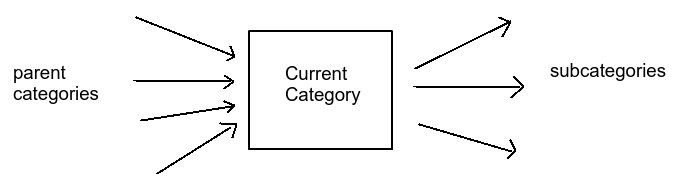
\includegraphics[width=\textwidth]{Chapters/Implementation/Grading/category_parent_sub}
\caption[Example of \emph{inlink} and \emph{outlink} for a category]{Example of how a category has links from parent categories and links to its subcategories. \emph{inlink} for the category is 4 and \emph{outlink} for the category is 3.}
\label{fig:Categorywparentandsub2}
\end{figure}

One assumption is that categories with high \emph{inlink} can be reached from categories that are not about the same. 

Another assumption is that categories with a high number for \emph{outlink} are more likely to reach articles not necessarily connected to the category name since they can reach far in all the subcategories' directions. Thus, categories with a high value of \emph{outlink} and a high value of \emph{inlink} should have a lower score than categories seldom reached. 

\subsubsection{Grading based on Inlinks and Outlinks}
The assumption that categories with high \emph{inlink} and \emph{outlink} are more often visited leads to the thought that these categories should have a lower score than categories that are more rarly visited. 

The first approach was therefore to find the \emph{inlink} and \emph{outlink} of all categories in the structure. These numbers had to be compared with the average number of \emph{inlink} and \emph{outlink} to know whether the number is high or low (see Table \ref{tab:avginlinkoutlink}). 

The score for each category was then 

\begin{equation} \label{eq:scoreinout}
Score_{C} = \frac{inlink_{c} + outlink_{c}}{\xoverline{C_{in}} + \xoverline{C_{out}}}
\end{equation}
where $\xoverline{C_{in}}$ is the average \emph{inlink} and $\xoverline{C_{out}}$ is the average \emph{outlink}.

The scoring from formula \ref{eq:scoreinout} means that paths with categories rarely visited will be favoured, hence given a lower score. 

\subsection{Normalized Grading based on Inlinks and Outlinks}
Grading based on \emph{inlink} and \emph{outlink} favorises short paths even if the paths contains categories considered bad. One way of handling this problem is by normalizing the score of each path. Equation \ref{eq:normscoreinput} is a way of normalizing the path score of path $P$ so the length of the path does not determine the relevance of the path. 

% TODO: Write something about normalization - why is it good for grading?

\begin{equation} \label{eq:normscoreinput}
Pathscore_{P} = \frac{1}{N} \sum_{c} Score_{C}
\end{equation}
where $N$ is number of categories in the path.


\subsection{Deciding Relevant Paths}
One way of deciding which graded paths are relevant are by choosing a threshold for the path score. If the score is lower than a given score, it is marked as relevant and higher score means that it is not relevant. A threshold can be found by deciding how many paths 

The way to do this is to find the scores of all paths. and sort the scores from lowest to highest (see \ref{eq:sortedscores}). Then a $k$ has to be decided to how many paths are believed relevant of all paths, for instance one could assume that only 10\% of the paths are relevant, which leads to$ k = .10 \cdot n$. 

\begin{equation} \label{eq:sortedscores}
Sorted\_scores = \left[ S_{1}, S_{2}, ... , S_{k}, ... , S_{n} \right]
\end{equation}



\begin{equation} \label{eq:threshold}
T = Sorted\_scores[k]
\end{equation}


The problem with this method is that not all articles are guaranteed to have any relevant paths. The other problem is that the score of the path will vary a lot within different fields, since some of the Wikipedia articles are categorized under very specified categories. 
% TODO: Finn en kilde som er enig med meg. 

% Problem: 
% Finne hvor mange pather som er tilgjengelig. 

Another approach is to choose the best $k$ paths for each Wikipedia article. This approach is independent of the values on other articles' path score which means all Wikipedia articles are guaranteed at least one path. The disadvantage is that some paths might be marked as relevant even though their path score is lower than path scores marked as irrelevant by other articles. Another disadvantage is that articles with many good paths will still have to choose the best $k$ paths and good paths might be lost. 

\begin{comment}
Fordeler: ser ikke på de andre
alle articler får minst en score. 

Ulemper: mange gode - hvilken er best?
Kan ikke vite om scoren er god

\end{comment}


\section{Evaluation}
The main purpose of the evaluation is to see whether there are any improvements when the results are applied. There are different ways of measuring 


Evaluation is the 